\subsubsubsubsection{Vehicle}
\begin{figure}[h]
\centering
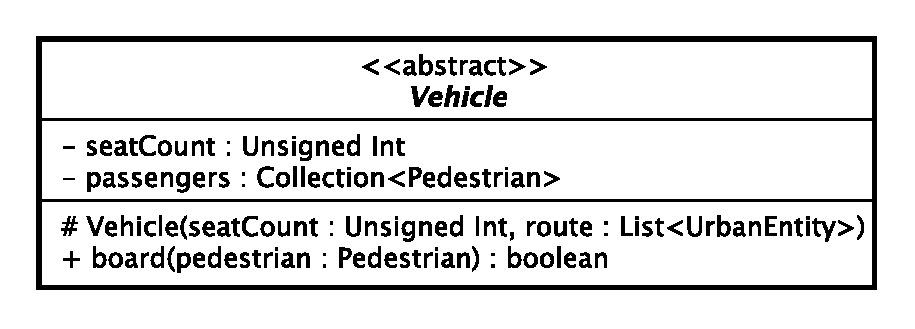
\includegraphics[scale=0.6,keepaspectratio]{images/solution/vehicle.eps}
\caption{App::Active::Vehicle}
\label{fig:sd-app-vehicle}
\end{figure}
\begin{itemize}
  \item \textbf{Description} \\
    It represents an entity that moves through the city carrying one or more
pedestrians.
  \item \textbf{Attribute}
  \begin{itemize}
    \item \texttt{- maxSeats: Unsigned Int} \\
The maximum number of seats in the vehicle.
    \item \texttt{- seat: ArrayList<Pedestrian>} \\
The list of passengers carried by the vehicle.
  \end{itemize}
  \item \textbf{Operation}
  \begin{itemize} 
    \item \texttt{+ board(passenger: Pedestrian) : boolean} \\
If the vehicle is not full the pedestrian become a passenger and the method returns \textit{true}.
Otherwise the access to the vehicle is not granted and the method returns false.
  \end{itemize}
\end{itemize}
